% ============================================================
%  Autoresearch 2.0 — Technical Blog Post
%  Author: Sovesh Mohapatra
%  Date:   March 2026
% ============================================================

\documentclass[12pt, a4paper]{article}

% ---------- Encoding & Fonts ----------
\usepackage[T1]{fontenc}
\usepackage[utf8]{inputenc}
\usepackage{lmodern}
\usepackage{microtype}

% ---------- Layout ----------
\usepackage[top=2.8cm, bottom=3cm, left=3cm, right=3cm]{geometry}
\usepackage{setspace}
\setstretch{1.25}
\usepackage{parskip}

% ---------- Colours ----------
\usepackage[dvipsnames]{xcolor}
\definecolor{brand}{HTML}{0A66C2}        % LinkedIn blue
\definecolor{darkbg}{HTML}{1A1A2E}       % dark terminal bg
\definecolor{codegreen}{HTML}{4EC9B0}
\definecolor{codeyellow}{HTML}{DCDCAA}
\definecolor{codepurple}{HTML}{C586C0}
\definecolor{codeorange}{HTML}{CE9178}
\definecolor{codelightblue}{HTML}{9CDCFE}
\definecolor{lightgray}{HTML}{F4F4F5}
\definecolor{warmgray}{HTML}{6B7280}
\definecolor{accent}{HTML}{E11D48}       % red accent
\definecolor{green}{HTML}{16A34A}

% ---------- Graphics ----------
\usepackage{graphicx}
\usepackage{tikz}
\usetikzlibrary{shapes.geometric, arrows.meta, positioning, fit,
                backgrounds, calc, decorations.pathmorphing,
                decorations.markings, shadows, matrix, chains}

% ---------- Tables ----------
\usepackage{booktabs}
\usepackage{tabularx}
\usepackage{multirow}
\usepackage{array}
\usepackage{colortbl}
\newcolumntype{C}{>{\centering\arraybackslash}X}

% ---------- Code Listings ----------
\usepackage{listings}
\lstdefinestyle{pythonstyle}{
  backgroundcolor=\color{darkbg},
  basicstyle=\ttfamily\footnotesize\color{white},
  keywordstyle=\color{codepurple}\bfseries,
  stringstyle=\color{codeorange},
  commentstyle=\color{warmgray}\itshape,
  numberstyle=\tiny\color{warmgray},
  breaklines=true,
  frame=none,
  numbers=left,
  numbersep=8pt,
  showstringspaces=false,
  tabsize=4,
  xleftmargin=12pt,
  xrightmargin=4pt,
  aboveskip=0pt,
  belowskip=0pt,
  morekeywords={True, False, None, import, from, def, class, return,
                if, else, elif, for, while, with, as, try, except,
                raise, pass, break, continue, and, or, not, in, is,
                lambda, yield, global, nonlocal, assert, del},
  literate={->}{{\textcolor{codepurple}{->}}}{2}
           {:=}{{\textcolor{codepurple}{:=}}}{2},
}

\lstdefinestyle{bashstyle}{
  backgroundcolor=\color{darkbg},
  basicstyle=\ttfamily\footnotesize\color{codegreen},
  breaklines=true,
  frame=none,
  showstringspaces=false,
  xleftmargin=12pt,
  xrightmargin=4pt,
  aboveskip=0pt,
  belowskip=0pt,
}

\lstdefinestyle{terminalstyle}{
  backgroundcolor=\color{darkbg},
  basicstyle=\ttfamily\footnotesize\color{white},
  breaklines=true,
  frame=none,
  showstringspaces=false,
  xleftmargin=12pt,
  xrightmargin=4pt,
  aboveskip=0pt,
  belowskip=0pt,
}

% ---------- tcolorbox ----------
\usepackage[most]{tcolorbox}

\tcbset{
  codebox/.style={
    colback=darkbg,
    colframe=warmgray!40,
    arc=4pt,
    boxrule=0.6pt,
    left=8pt, right=8pt, top=6pt, bottom=6pt,
    fonttitle=\ttfamily\small\bfseries\color{warmgray},
    title={},
  },
  callout/.style={
    colback=#1!8,
    colframe=#1!60,
    arc=6pt,
    boxrule=0.8pt,
    left=10pt, right=10pt, top=8pt, bottom=8pt,
  },
  statcard/.style={
    colback=white,
    colframe=brand!40,
    arc=8pt,
    boxrule=1pt,
    shadow={1.5mm}{-1.5mm}{0mm}{black!10},
    left=10pt, right=10pt, top=10pt, bottom=10pt,
  },
}

% ---------- Sectioning Style ----------
\usepackage{titlesec}
\titleformat{\section}{\Large\bfseries\color{darkbg}}{}{0em}{}[\vspace{-4pt}\rule{\linewidth}{2pt}]
\titleformat{\subsection}{\large\bfseries\color{brand}}{}{0em}{}
\titleformat{\subsubsection}{\normalsize\bfseries\color{darkbg}}{}{0em}{}
\titlespacing{\section}{0pt}{18pt}{8pt}
\titlespacing{\subsection}{0pt}{12pt}{4pt}

% ---------- Hyperref ----------
\usepackage[colorlinks=true, linkcolor=brand, urlcolor=brand, citecolor=accent]{hyperref}

% ---------- Math ----------
\usepackage{amsmath, amssymb}

% ---------- Misc ----------
\usepackage{enumitem}
\usepackage{float}
\usepackage{caption}
\captionsetup{font=small, labelfont=bf, textfont=it, skip=6pt}
\usepackage{subcaption}
\usepackage{mdframed}
\usepackage{fontawesome5}

% ============================================================
%  Custom Commands
% ============================================================
\newcommand{\bpb}{\texttt{val\_bpb}}
\newcommand{\trainpy}{\texttt{train.py}}
\newcommand{\file}[1]{\texttt{#1}}
\newcommand{\flag}[1]{\texttt{--#1}}
\newcommand{\code}[1]{\texttt{#1}}
\newcommand{\metric}[2]{\textbf{#1}~\textcolor{warmgray}{(#2)}}

% Inline coloured badge
\newcommand{\badge}[2]{%
  \tikz[baseline=(n.base)]\node[fill=#1, text=white, rounded corners=3pt,
  inner sep=2pt 4pt, font=\ttfamily\scriptsize\bfseries](n){#2};%
}

% ============================================================
%  Title
% ============================================================
\title{%
  {\color{darkbg}\Huge\bfseries Autoresearch 2.0}\\[6pt]
  {\large\color{warmgray} How I Built a Self-Improving Language Model Lab\\
  That Runs~100~Experiments While You Sleep}\\[4pt]
  \rule{\linewidth}{0.6pt}
}
\author{%
  \textbf{Sovesh Mohapatra}\\
  \small\color{warmgray}
  \href{https://www.linkedin.com/in/soveshmohapatra}{linkedin.com/in/soveshmohapatra}~~|~~
  \href{https://github.com/soveshmohapatra/autoresearch-2.0}{github.com/soveshmohapatra/autoresearch-2.0}
}
\date{March 2026}

% ============================================================
\begin{document}
\maketitle
\thispagestyle{empty}

% ============================================================
%  Hero Pull-Quote
% ============================================================
\begin{tcolorbox}[callout=brand, halign=center]
\itshape\large
``One day, frontier AI research used to be done by meat computers in between eating, sleeping,
having other fun\ldots That era is long gone.''\\[4pt]
\normalfont\small\color{warmgray}--- @karpathy, March 2026
\end{tcolorbox}

\vspace{8pt}

% ============================================================
%  Stat Cards Row
% ============================================================
\noindent
\begin{minipage}[t]{0.32\linewidth}
\begin{tcolorbox}[statcard, halign=center]
  {\fontsize{28}{32}\selectfont\bfseries\color{brand} 10}\\[2pt]
  {\small\color{warmgray} Languages}
\end{tcolorbox}
\end{minipage}\hfill
\begin{minipage}[t]{0.32\linewidth}
\begin{tcolorbox}[statcard, halign=center]
  {\fontsize{28}{32}\selectfont\bfseries\color{brand} $\sim$12}\\[2pt]
  {\small\color{warmgray} Experiments / Hour}
\end{tcolorbox}
\end{minipage}\hfill
\begin{minipage}[t]{0.32\linewidth}
\begin{tcolorbox}[statcard, halign=center]
  {\fontsize{28}{32}\selectfont\bfseries\color{brand} $\sim$100}\\[2pt]
  {\small\color{warmgray} Experiments Overnight}
\end{tcolorbox}
\end{minipage}

\vspace{16pt}
\tableofcontents
\newpage

% ============================================================
\section{Introduction}
% ============================================================

What if you could run 100 machine learning experiments while you slept, and wake up to a model
that had autonomously improved itself overnight?

That is not a hypothetical. That is exactly what \textbf{Autoresearch~2.0} does.

This project started as my adaptation of
\href{https://github.com/karpathy/autoresearch}{karpathy/autoresearch} by Andrej Karpathy.
The original concept is elegant: train a small GPT-style language model with a fixed time
budget, measure a vocabulary-size-independent metric (\bpb{}), and let an AI agent propose and
test architectural changes one by one in a tight loop.

I took that skeleton and rebuilt it into something more powerful:

\begin{itemize}[leftmargin=*, itemsep=2pt]
  \item A full architecture variant zoo (MoE, GQA, SwiGLU, Pre-norm)
  \item A three-optimizer toolkit (Muon+AdamW, Lion, Adafactor)
  \item \textbf{Bayesian hyperparameter search} via Optuna, embedded directly in \trainpy{}
  \item \textbf{Smart checkpoint management}: only best + latest, never accumulates stale files
  \item Support for \textbf{10 languages} with isolated per-language caches
  \item A live terminal dashboard with loss sparklines
  \item Full CUDA / Apple Silicon / CPU support with auto-detected hardware caps
\end{itemize}

The rest of this post explains how every piece works, from the attention mechanism to the
autonomous agent loop.

% ============================================================
\section{Why \texttt{val\_bpb}? The Vocabulary-Independent Metric}
% ============================================================

Standard language model evaluation reports cross-entropy loss, which is tied to vocabulary
size. Doubling the vocabulary roughly halves the loss, making experiments across different
tokenisers incomparable.

Bits-per-byte (\bpb{}) sidesteps this by measuring information per \emph{raw byte} of text:

\begin{equation}
  \text{bpb} = \frac{\mathcal{L}_{\text{CE}}}{\log(2) \cdot \bar{b}}
  \label{eq:bpb}
\end{equation}

where $\mathcal{L}_{\text{CE}}$ is the cross-entropy loss and $\bar{b}$ is the average number
of bytes per token for the given tokeniser. Lower is better. A perfect character-level
model on English achieves roughly 1.0~bpb.

This makes every experiment in the loop directly comparable regardless of architecture size or
tokeniser — a critical property when the agent explores hundreds of configurations.

% ============================================================
\section{System Architecture}
% ============================================================

\begin{figure}[H]
\centering
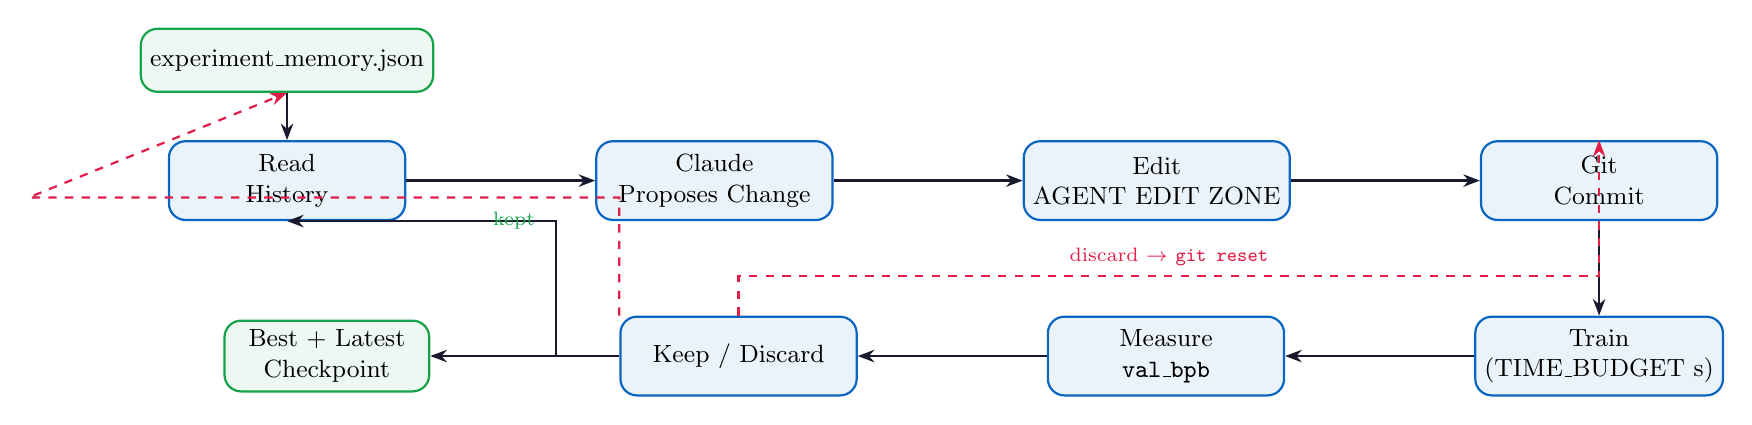
\begin{tikzpicture}[
  node distance=1.6cm and 2.4cm,
  every node/.style={font=\small},
  box/.style={draw=brand, fill=brand!8, rounded corners=6pt, minimum height=1cm,
              minimum width=3cm, align=center, thick},
  agent/.style={draw=accent, fill=accent!8, rounded corners=6pt, minimum height=1cm,
               minimum width=3cm, align=center, thick},
  store/.style={draw=green, fill=green!8, rounded corners=6pt, minimum height=0.8cm,
               minimum width=2.6cm, align=center, thick},
  arrow/.style={-{Stealth[length=6pt]}, thick, color=darkbg},
  darrow/.style={-{Stealth[length=6pt]}, thick, color=accent, dashed},
]

% Row 1 — core pipeline
\node[box] (history)  {Read\\History};
\node[box, right=of history] (propose) {Claude\\Proposes Change};
\node[box, right=of propose] (edit)    {Edit\\AGENT EDIT ZONE};
\node[box, right=of edit]    (commit)  {Git\\Commit};

% Row 2 — training
\node[box, below=1.2cm of commit] (train)  {Train\\(TIME\_BUDGET s)};
\node[box, left=of train]         (eval)   {Measure\\\bpb{}};
\node[box, left=of eval]          (decide) {Keep / Discard};
\node[store, left=of decide]      (ckpt)   {Best + Latest\\Checkpoint};

% Arrows — top row
\draw[arrow] (history) -- (propose);
\draw[arrow] (propose) -- (edit);
\draw[arrow] (edit)    -- (commit);
\draw[arrow] (commit)  -- (train);

% Arrows — bottom row
\draw[arrow] (train)  -- (eval);
\draw[arrow] (eval)   -- (decide);
\draw[arrow] (decide) -- (ckpt);

% Feedback arrow
\draw[arrow] (decide.west) -- ++(-0.8,0) |- (history.south)
  node[midway, left, xshift=-4pt, text=green]{\scriptsize kept};

% Discard arrow
\draw[darrow] (decide.north) -- ++(0,0.5) -| (commit.north)
  node[near start, above, text=accent]{\scriptsize discard $\to$ \texttt{git reset}};

% Experiment memory store
\node[store, above=0.6cm of history] (mem) {experiment\_memory.json};
\draw[arrow] (mem.south) -- (history.north);
\draw[darrow] (decide.north west) -- ++(0,1.5) -- ++(-7.5,0) -- (mem.south);

\end{tikzpicture}
\caption{The Autoresearch 2.0 experiment loop. Every cycle proposes one change,
trains for a fixed wall-clock budget, keeps improvements, and reverts regressions.}
\label{fig:loop}
\end{figure}

The system has five cooperating components:

\begin{center}
\begin{tabularx}{\linewidth}{@{}lX@{}}
\toprule
\textbf{File} & \textbf{Role} \\
\midrule
\file{train.py}    & GPT model, training loop, AGENT EDIT ZONE, Optuna HPO \\
\file{agent.py}    & Claude API loop: reads history, proposes change, edits \trainpy{} \\
\file{run\_loop.py}& Orchestrator: git commit $\to$ train $\to$ measure $\to$ keep/discard \\
\file{prepare.py}  & Data download, BPE tokeniser, \bpb{} evaluation \\
\file{gui.py}      & Rich terminal dashboard with live loss sparkline \\
\file{config.py}   & Hardware-aware configuration dataclass \\
\file{hardware.py} & CUDA / MPS / CPU detection and capability negotiation \\
\bottomrule
\end{tabularx}
\end{center}

% ============================================================
\section{The GPT Transformer — What's Inside}
% ============================================================

The model is a standard GPT-2-style causal language model, built from scratch in PyTorch with
optional modern enhancements.

\subsection{Base Architecture}

\begin{figure}[H]
\centering
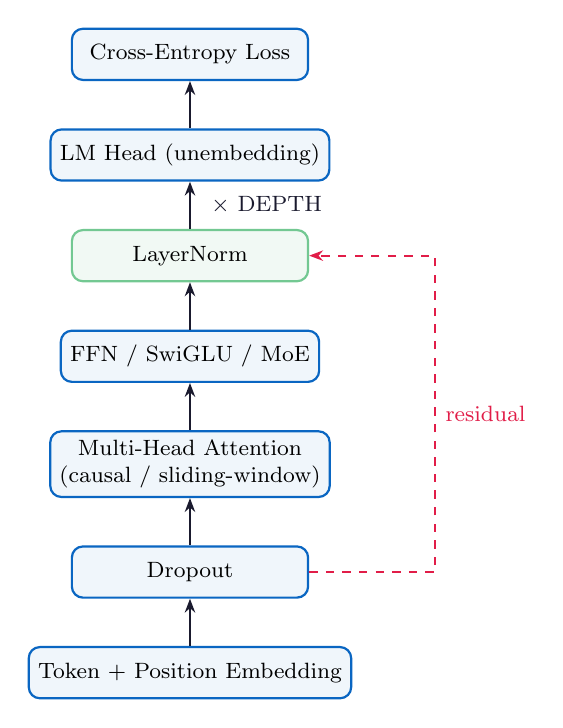
\begin{tikzpicture}[
  every node/.style={font=\footnotesize},
  block/.style={draw=brand, fill=brand!6, rounded corners=4pt, minimum width=3cm,
                minimum height=0.65cm, align=center, thick},
  arrow/.style={-{Stealth[length=5pt]}, thick, color=darkbg},
]

\node[block] (embed)    {Token + Position Embedding};
\node[block, above=0.6cm of embed] (drop)  {Dropout};
\node[block, above=0.6cm of drop]  (attn)  {Multi-Head Attention\\(causal / sliding-window)};
\node[block, above=0.6cm of attn]  (mlp)   {FFN / SwiGLU / MoE};
\node[draw=green!60, fill=green!6, rounded corners=4pt, minimum width=3cm,
      minimum height=0.65cm, align=center, thick, above=0.6cm of mlp] (ln)   {LayerNorm};
\node[block, above=0.6cm of ln]    (head)  {LM Head (unembedding)};
\node[block, above=0.6cm of head]  (loss)  {Cross-Entropy Loss};

\draw[arrow] (embed) -- (drop);
\draw[arrow] (drop)  -- (attn);
\draw[arrow] (attn)  -- (mlp);
\draw[arrow] (mlp)   -- (ln);
\draw[arrow] (ln)    -- (head) node[midway, right, xshift=4pt]{$\times$ DEPTH};
\draw[arrow] (head)  -- (loss);

% Residual connection for one block
\draw[arrow, color=accent, dashed]
  (drop.east) -- ++(1.6,0) |- (ln.east)
  node[near start, right, text=accent]{residual};

\end{tikzpicture}
\caption{One transformer block (repeated DEPTH times). With \code{USE\_PRENORM=True} the
LayerNorm moves before the attention and FFN sublayers.}
\label{fig:transformer}
\end{figure}

The architecture is parametrised by just three numbers:

\begin{equation}
  d_{\text{model}} = \text{DEPTH} \times \text{ASPECT\_RATIO}, \qquad
  n_{\text{heads}} = d_{\text{model}} / \text{HEAD\_DIM}
\end{equation}

This coupling means adding a layer also widens the model, mimicking the depth-to-width ratio
of models like GPT-2 (depth~12, width~768, ratio~64).

\subsection{Sliding-Window Attention (WINDOW\_PATTERN)}

Not every layer needs full $O(n^2)$ attention. The \code{WINDOW\_PATTERN} string controls
which layers use full context (\code{L}) and which use half-context sliding windows (\code{S}):

\begin{center}
\begin{tabular}{@{}lll@{}}
\toprule
\textbf{Pattern} & \textbf{Meaning} & \textbf{When to use} \\
\midrule
\code{"SSSL"} & 3 sliding + 1 full (default) & Efficient, good local context \\
\code{"LLLL"} & All full attention & When local patterns plateau \\
\code{"SSSS"} & All sliding window & Maximum speed / long sequences \\
\code{"SLLL"} & 1 sliding + 3 full & Intermediate \\
\bottomrule
\end{tabular}
\end{center}

\subsection{Architecture Variants}

The AGENT EDIT ZONE exposes five boolean flags:

\begin{tcolorbox}[codebox, title=Architecture Variant Flags]
\begin{lstlisting}[style=pythonstyle]
USE_MOE          = False   # Sparse Mixture-of-Experts FFN
USE_GQA          = False   # Grouped Query Attention
USE_SWIGLU       = False   # SwiGLU activation (vs ReLU^2)
USE_PRENORM      = False   # Pre-norm residual stream
USE_WEIGHT_TYING = False   # Tie lm_head <-> wte weights
\end{lstlisting}
\end{tcolorbox}

\subsubsection{SwiGLU Activation}

The standard FFN uses a squared ReLU: $\text{ReLU}(x)^2$. SwiGLU replaces it with a gated
variant:

\begin{equation}
  \text{SwiGLU}(x) = \bigl(\text{Swish}(W_1 x)\bigr) \odot (W_2 x),
  \qquad \text{Swish}(z) = z \cdot \sigma(z)
\end{equation}

Despite effectively halving the hidden dimension (the gate and value paths each get
$2\times$ the normal expansion), SwiGLU consistently improves perplexity at typical
nano-model scales.

\subsubsection{Grouped Query Attention (GQA)}

Standard multi-head attention has $n_{\text{heads}}$ separate KV projections. GQA reduces
this to $n_{\text{heads}} / \text{GQA\_KV\_GROUPS}$ shared KV heads, slashing the KV cache
footprint:

\begin{equation}
  \text{KV memory} = 2 \cdot L \cdot n_{\text{kv}} \cdot d_{\text{head}} \cdot \text{bytes}
\end{equation}

This lets you fit a deeper or wider model in the same VRAM envelope — critical on consumer
GPUs.

\subsubsection{Mixture of Experts (MoE)}

MoE replaces the dense FFN with a sparse ensemble of $E$ experts, routing each token to
the top-$k$ experts:

\begin{equation}
  \text{MoE}(x) = \sum_{i \in \text{top-}k} g_i(x) \cdot \text{FFN}_i(x),
  \qquad \sum_i g_i = 1
\end{equation}

With \code{MOE\_NUM\_EXPERTS=4, MOE\_TOP\_K=2}, each token activates 2 of 4 experts — doubling
parameter count at roughly constant per-token FLOPs. Best on H100/A100 due to memory bandwidth.

% ============================================================
\section{The Optimizer Zoo}
% ============================================================

Three optimizers are available, each suited to different compute regimes.

\subsection{Muon + AdamW (Default)}

Muon (\emph{Momentum + Newton-Schulz orthogonalisation}) applies Nesterov momentum to
2D parameter matrices after projecting the gradient update onto the orthogonal group.
For weight matrices $W$:

\begin{equation}
  G_t = \text{NS}_5(M_t), \qquad W_{t+1} = W_t - \eta_{\text{matrix}} \cdot G_t
\end{equation}

where $\text{NS}_5$ denotes 5 iterations of Newton-Schulz iteration to compute an
approximate orthogonal polar factor. This gives update steps whose singular values are all
equal — a form of spectral normalisation that empirically accelerates training on transformer
weight matrices. Embeddings and scalars use standard AdamW.

\subsection{Lion}

Lion uses sign gradient descent with EMA:

\begin{equation}
  m_t = \beta_1 m_{t-1} + (1-\beta_1)g_t, \qquad
  W_{t+1} = W_t - \eta \cdot \text{sign}(m_t)
\end{equation}

Benefits: identical update magnitude per parameter (no second-moment accumulation),
roughly 3$\times$ smaller memory than Adam. Trade-off: more sensitive to learning rate.

\subsection{Adafactor}

Adafactor decomposes the second-moment matrix into row and column factors, dropping from
$O(n^2)$ to $O(n + m)$ memory for an $n \times m$ matrix. Useful when VRAM is the binding
constraint.

\begin{center}
\begin{tabular}{@{}llll@{}}
\toprule
\textbf{Optimizer} & \textbf{Memory} & \textbf{Speed} & \textbf{Best for} \\
\midrule
Muon+AdamW & $\sim$2$\times$ params & Fastest convergence & Default / CUDA \\
Lion       & $\sim$1.5$\times$ params & Fast, noisy & Memory-constrained \\
Adafactor  & $\sim$1.1$\times$ params & Slowest & Extreme VRAM limits \\
\bottomrule
\end{tabular}
\end{center}

% ============================================================
\section{The AGENT EDIT ZONE — One Section, All Experiments}
% ============================================================

The core design principle is \textbf{one file, one section}. The agent never touches anything
outside the clearly demarcated zone:

\begin{tcolorbox}[codebox, title=train.py — AGENT EDIT ZONE]
\begin{lstlisting}[style=pythonstyle]
# ================================================================
# AGENT EDIT ZONE
# This is the only section the agent (or you) ever modifies.
# ================================================================

# --- Model architecture ---
DEPTH         = 8           # transformer layers
ASPECT_RATIO  = 64          # model_dim = depth x aspect_ratio
HEAD_DIM      = 128         # attention head dimension
WINDOW_PATTERN = "SSSL"     # L=full context, S=half context

# --- Architecture variants ---
USE_MOE          = False    # Mixture of Experts
USE_GQA          = False    # Grouped Query Attention
USE_SWIGLU       = False    # SwiGLU activation
USE_PRENORM      = False    # Pre-norm residual stream
USE_WEIGHT_TYING = False    # Tie lm_head <-> wte

# --- Optimizer ---
OPTIMIZER_TYPE = "muon_adamw"   # "muon_adamw" | "lion" | "adafactor"
MATRIX_LR      = 0.04
WEIGHT_DECAY   = 0.2

# --- Training ---
TIME_BUDGET       = 300     # seconds per experiment (wall clock)
TOTAL_BATCH_SIZE  = 2**19   # ~524K tokens per step
DEVICE_BATCH_SIZE = 128     # reduce if OOM
GRAD_CLIP         = 1.0

# ================================================================
# END AGENT EDIT ZONE
# ================================================================
\end{lstlisting}
\end{tcolorbox}

Every experiment commits exactly this section. The git log becomes a perfect audit trail
of every hypothesis tested. Any regression rolls back with a single \code{git reset
--hard}.

% ============================================================
\section{The Autonomous Agent (agent.py)}
% ============================================================

\subsection{How It Works}

The agent is a tight loop powered by \textbf{Claude claude-opus-4-6}:

\begin{figure}[H]
\centering
\begin{tikzpicture}[
  every node/.style={font=\footnotesize},
  step/.style={draw=brand, fill=brand!8, rounded corners=5pt, minimum width=5.2cm,
               minimum height=0.7cm, align=center, thick},
  arrow/.style={-{Stealth[length=5pt]}, thick, color=darkbg},
  label/.style={font=\scriptsize\itshape, color=warmgray},
]

\node[step] (s1) {1. Read \texttt{experiment\_memory.json} + current EDIT ZONE};
\node[step, below=0.5cm of s1] (s2) {2. Send to Claude: history, zone, device info};
\node[step, below=0.5cm of s2] (s3) {3. Claude responds: DESCRIPTION + new EDIT ZONE};
\node[step, below=0.5cm of s3] (s4) {4. Parse response, apply edit to \texttt{train.py}};
\node[step, below=0.5cm of s4] (s5) {5. \texttt{git commit -m "experiment: <description>"}};
\node[step, below=0.5cm of s5] (s6) {6. \texttt{run\_loop.py --auto}: train + measure};
\node[step, below=0.5cm of s6] (s7) {7. val\_bpb improved? Keep. Else: \texttt{git reset}};
\node[step, below=0.5cm of s7] (s8) {8. Record to memory. Go to 1.};

\foreach \a/\b in {s1/s2, s2/s3, s3/s4, s4/s5, s5/s6, s6/s7, s7/s8}
  \draw[arrow] (\a) -- (\b);

% Feedback
\draw[arrow, color=accent, dashed, rounded corners=6pt]
  (s8.east) -- ++(1.5,0) |- (s1.east);
\node[label, right=1.6cm of s5] {$\sim$5 min/cycle};

\end{tikzpicture}
\caption{Agent loop: one Claude API call per experiment, one commit per change.}
\label{fig:agent}
\end{figure}

\subsection{The System Prompt}

Claude receives a strict system prompt that enforces scientific discipline:

\begin{tcolorbox}[callout=accent]
\small
\textbf{Rules the agent must follow:}
\begin{itemize}[itemsep=0pt, leftmargin=16pt]
  \item Change \textbf{exactly one} thing per experiment
  \item Keep all other constants at current values
  \item Never add code outside the AGENT EDIT ZONE
  \item On MPS: DEPTH$\leq$4, ASPECT\_RATIO$\leq$32, DEVICE\_BATCH\_SIZE$\leq$4 are hard limits
  \item Respond with \emph{only} DESCRIPTION and new EDIT ZONE (no extra text)
\end{itemize}
\end{tcolorbox}

This single-change discipline is key: it makes each experiment \emph{interpretable}.
You always know exactly why a model improved or regressed.

\subsection{Response Parsing}

The agent parses Claude's output with a regex that extracts the AGENT EDIT ZONE from a
Python code block, then applies it via a targeted search-and-replace — leaving all other
code in \trainpy{} untouched.

% ============================================================
\section{Optuna Hyperparameter Search — Bayesian HPO in One Flag}
% ============================================================

The single most impactful addition in Autoresearch 2.0 is \textbf{Bayesian hyperparameter
optimisation} via Optuna, embedded directly in \trainpy{}.

\begin{tcolorbox}[codebox, title=Usage]
\begin{lstlisting}[style=bashstyle]
# Run 20 trials (Bayesian, 300s each) — default
uv run python train.py --optuna

# 50 trials, 120s budget, Hindi corpus
uv run python train.py --optuna --trials 50 --time-budget 120 --language hi

# Resume a previous study from SQLite DB
uv run python train.py --optuna --optuna-resume

# Print best params and reproduce command, then exit
uv run python train.py --best
\end{lstlisting}
\end{tcolorbox}

\subsection{How Optuna Is Wired In}

Optuna lives in an \textbf{early-exit block} at the very top of \trainpy{}, immediately
after argument parsing:

\begin{tcolorbox}[codebox, title=train.py — Optuna early-exit (simplified)]
\begin{lstlisting}[style=pythonstyle]
args = parse_args()

if args.optuna or args.best:
    import optuna
    from optuna.samplers import TPESampler
    from optuna.pruners import MedianPruner

    _sampler = TPESampler(seed=42, n_startup_trials=5)
    _pruner  = MedianPruner(n_startup_trials=5)
    _study = optuna.create_study(
        study_name=args.study_name,
        storage="sqlite:///optuna_study.db",
        direction="minimize",
        sampler=_sampler,
        pruner=_pruner,
        load_if_exists=True,   # resume if DB exists
    )

    def _objective(trial):
        params = _suggest(trial)      # sample hyper-params
        cmd = _build_cmd(params, ...) # build subprocess command
        subprocess.run(cmd, ...)      # run train.py WITHOUT --optuna
        bpb = _parse_bpb("run.log")  # parse val_bpb from output
        return bpb                    # Optuna minimises this

    _study.optimize(_objective, n_trials=args.trials)
    _print_best(_study)
    sys.exit(0)                        # normal training path untouched
\end{lstlisting}
\end{tcolorbox}

The normal training path below this block is completely unaffected — no conditional spaghetti,
no import-time side effects.

\subsection{The Search Space}

\begin{center}
\begin{tabular}{@{}lll@{}}
\toprule
\textbf{Parameter} & \textbf{Type} & \textbf{Range / Choices} \\
\midrule
\code{depth}          & int (step 2)  & 2 -- 10 \\
\code{aspect\_ratio}  & categorical   & 32, 48, 64, 96 \\
\code{head\_dim}      & categorical   & 64, 128 \\
\code{optimizer\_type}& categorical   & muon\_adamw, lion, adafactor \\
\code{matrix\_lr}     & log-uniform   & 0.005 -- 0.1 \\
\code{weight\_decay}  & log-uniform   & 0.05 -- 0.5 \\
\code{use\_swiglu}    & boolean       & True / False \\
\code{use\_prenorm}   & boolean       & True / False \\
\code{use\_weight\_tying} & boolean   & True / False \\
\bottomrule
\end{tabular}
\end{center}

\subsection{TPE Sampler — Why Bayesian?}

Random search treats each trial independently. The \textbf{Tree-structured Parzen Estimator
(TPE)} builds two density models after each trial:
$\ell(x)$ for configurations that performed better than a threshold, and $g(x)$ for the rest.
The next trial samples from $\arg\max \ell(x)/g(x)$ — concentrating search in promising
regions.

\begin{figure}[H]
\centering
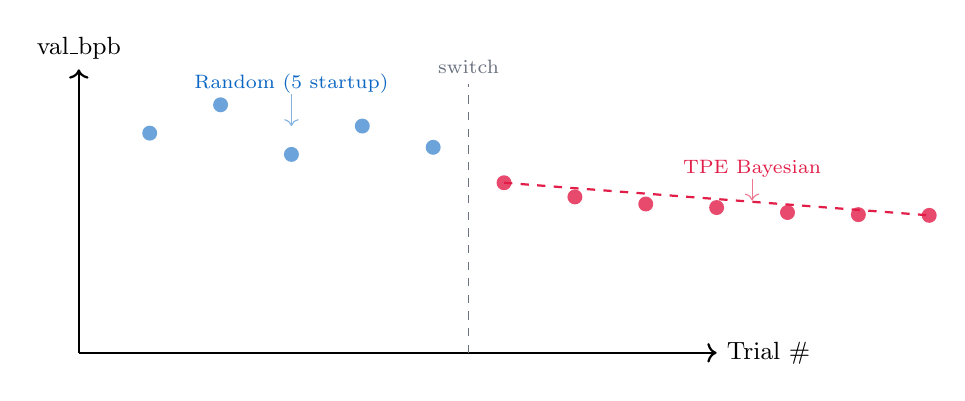
\begin{tikzpicture}[scale=0.9]
% Axes
\draw[thick,->] (0,0) -- (9,0) node[right]{\small Trial \#};
\draw[thick,->] (0,0) -- (0,4) node[above]{\small val\_bpb};

% Random phase (trials 1-5) — noisy high bpb
\foreach \x/\y in {1/3.1, 2/3.5, 3/2.8, 4/3.2, 5/2.9}
  \fill[brand!60] (\x,\y) circle(3pt);

% TPE phase (trials 6+) — converging lower
\foreach \x/\y in {6/2.4, 7/2.2, 8/2.1, 9/2.05, 10/1.98, 11/1.95, 12/1.94}
  \fill[accent!80] (\x,\y) circle(3pt);

% Trend line TPE
\draw[accent, thick, dashed] (6,2.4) -- (12,1.94);

% Annotations
\node[brand, font=\scriptsize] at (3, 3.8) {Random (5 startup)};
\draw[brand!50, ->] (3,3.65) -- (3,3.2);

\node[accent, font=\scriptsize] at (9.5, 2.6) {TPE Bayesian};
\draw[accent!60, ->] (9.5,2.45) -- (9.5,2.15);

% Dashed vertical line
\draw[warmgray, dashed] (5.5,0) -- (5.5,3.8)
  node[above, font=\scriptsize, color=warmgray]{switch};
\end{tikzpicture}
\caption{TPE transitions from random exploration to Bayesian exploitation after
\texttt{n\_startup\_trials=5}. bpb converges faster than pure random search.}
\label{fig:optuna}
\end{figure}

Results are persisted in \file{optuna\_study.db} (SQLite) and \file{optuna\_trials.jsonl}
(human-readable), so any interrupted study can be resumed with \flag{optuna-resume}.

% ============================================================
\section{Smart Checkpoint Management}
% ============================================================

A subtle but important fix over the original: checkpoint managers that start with an
empty list are blind to checkpoints from previous runs, leading to unbounded disk usage.

\subsection{The Bug}

\begin{tcolorbox}[callout=accent, title=Before: silent disk accumulation]
\begin{lstlisting}[style=pythonstyle]
class CheckpointManager:
    def __init__(self, save_dir, keep_last=3):
        self.checkpoints = []   # <-- WRONG: ignores existing .pt files
\end{lstlisting}
\end{tcolorbox}

Each run started with an empty list, so the pruning loop never saw old checkpoints.
After 20 experiments with 3 checkpoints each, you had 60 files on disk.

\subsection{The Fix: Scan Disk on Init}

\begin{tcolorbox}[codebox, title=After: disk-aware initialisation]
\begin{lstlisting}[style=pythonstyle]
class CheckpointManager:
    def __init__(self, save_dir, enabled=True):
        self.save_dir = Path(save_dir)
        self.enabled  = enabled
        if self.enabled:
            self.save_dir.mkdir(parents=True, exist_ok=True)
            self.checkpoints = sorted(
                self.save_dir.glob("checkpoint_*.pt"),
                key=lambda p: p.stat().st_mtime,
            )
        else:
            self.checkpoints = []
\end{lstlisting}
\end{tcolorbox}

\subsection{Best + Latest Retention Policy}

Instead of keeping the last $N$ by time (which discards the best model once training
improves further), we keep exactly two files:

\begin{tcolorbox}[codebox, title=\_prune: keep only best + latest]
\begin{lstlisting}[style=pythonstyle]
def _bpb_from_path(self, p: Path) -> float:
    try:
        return float(p.stem.split("_bpb")[-1])
    except Exception:
        return float("inf")

def _prune(self):
    if len(self.checkpoints) <= 2:
        return
    best   = min(self.checkpoints, key=self._bpb_from_path)
    latest = self.checkpoints[-1]
    keep   = {best, latest}
    for ckpt in list(self.checkpoints):
        if ckpt not in keep and ckpt.exists():
            ckpt.unlink()
            self.checkpoints.remove(ckpt)
\end{lstlisting}
\end{tcolorbox}

Checkpoint filenames encode the metric: \code{checkpoint\_step12400\_bpb1.8234.pt}.
This makes the best checkpoint trivially identifiable without loading any files.

\begin{figure}[H]
\centering
\begin{tikzpicture}[
  every node/.style={font=\scriptsize},
  ckpt/.style={draw=brand!60, fill=brand!8, rounded corners=3pt,
               minimum width=3.8cm, minimum height=0.55cm, align=center},
  del/.style={draw=accent!60, fill=accent!8, rounded corners=3pt,
              minimum width=3.8cm, minimum height=0.55cm, align=center},
  arrow/.style={-{Stealth[length=4pt]}, color=darkbg},
]
% Timeline
\node[ckpt] (c1) at (0,0)   {\texttt{step1000\_bpb2.41}};
\node[del]  (c2) at (0,-0.8){\texttt{step2000\_bpb2.18}};
\node[del]  (c3) at (0,-1.6){\texttt{step3000\_bpb2.05}};
\node[ckpt] (c4) at (0,-2.4){\texttt{step4000\_bpb1.92} \textcolor{green}{\faIcon{trophy} best}};
\node[del]  (c5) at (0,-3.2){\texttt{step5000\_bpb1.94}};
\node[ckpt] (c6) at (0,-4.0){\texttt{step6000\_bpb1.96} \textcolor{brand}{\faIcon{clock} latest}};

% Annotations
\node[right=0.3cm of c2, text=accent]{\faIcon{trash} pruned};
\node[right=0.3cm of c3, text=accent]{\faIcon{trash} pruned};
\node[right=0.3cm of c5, text=accent]{\faIcon{trash} pruned};
\node[right=0.3cm of c1, text=warmgray]{kept (first)};
\end{tikzpicture}
\caption{After 6 saves, only the best (\texttt{bpb1.92}) and latest (\texttt{bpb1.96})
checkpoints survive. All others are deleted automatically.}
\label{fig:ckpt}
\end{figure}

% ============================================================
\section{Multi-Language Support}
% ============================================================

Each of the 10 supported languages gets a fully isolated file tree under
\code{\textasciitilde/.cache/autoresearch/\{lang\}/}:

\begin{tcolorbox}[codebox]
\begin{lstlisting}[style=terminalstyle]
~/.cache/autoresearch/
  en/
    data/           <- Wikipedia token shards
    tokenizer/      <- BPE vocab (8192 tokens, trained on lang data)
    checkpoints/    <- best + latest .pt files
    meta.json       <- shard metadata
  hi/               <- identical structure for Hindi
  zh/               <- ... Chinese
  or/               <- ... Odia
  ...
\end{lstlisting}
\end{tcolorbox}

\begin{center}
\begin{tabular}{@{}clclcl@{}}
\toprule
  & \textbf{Code} & \textbf{Language}
& & \textbf{Code} & \textbf{Language} \\
\midrule
\badge{brand}{en} & \code{en} & English
& \badge{brand}{ja} & \code{ja} & Japanese \\
\badge{brand}{fr} & \code{fr} & French
& \badge{brand}{gu} & \code{gu} & Gujarati \\
\badge{brand}{es} & \code{es} & Spanish
& \badge{brand}{nl} & \code{nl} & Dutch \\
\badge{brand}{de} & \code{de} & German
& \badge{brand}{or} & \code{or} & Odia \\
\badge{brand}{hi} & \code{hi} & Hindi
& \badge{brand}{zh} & \code{zh} & Chinese \\
\bottomrule
\end{tabular}
\end{center}

The tokeniser is trained from scratch on each language's Wikipedia data using BPE with a
fixed vocabulary size of 8,192 tokens, ensuring the tokeniser genuinely reflects the
morphology of each language rather than defaulting to an English-dominated vocabulary.

% ============================================================
\section{Platform Support and Hardware Caps}
% ============================================================

\begin{center}
\begin{tabular}{@{}lcccc@{}}
\toprule
\textbf{Platform} & \texttt{compile} & \textbf{Flash Attn 3} & \textbf{Dtype} & \textbf{Rec.\ Batch} \\
\midrule
CUDA H100          & \checkmark & \checkmark~Hopper & bfloat16 & 128--256 \\
CUDA A100          & \checkmark & \checkmark        & bfloat16 & 64--128  \\
CUDA RTX 4090      & \checkmark & \checkmark        & bfloat16 & 32--64   \\
Apple M-Max/Ultra  & \checkmark* & \texttimes       & bfloat16 & 16--32   \\
Apple M-Base       & \checkmark* & \texttimes       & bfloat16 & 4 (auto-capped) \\
CPU                & \texttimes & \texttimes        & float32  & 4        \\
\bottomrule
\multicolumn{5}{l}{\small *Requires PyTorch $\geq$ 2.3 and macOS $\geq$ 14.4}
\end{tabular}
\end{center}

Apple Silicon (MPS) gets automatic hard caps to fit within the shared memory pool:

\begin{tcolorbox}[codebox]
\begin{lstlisting}[style=pythonstyle]
if DEVICE == "mps":
    os.environ["PYTORCH_ENABLE_MPS_FALLBACK"] = "1"
    os.environ["PYTORCH_MPS_HIGH_WATERMARK_RATIO"] = "0.0"
    config.training.device_batch_size = 4
    config.training.total_batch_size  = 2**14
    config.model.depth       = 4
    config.model.aspect_ratio = 32
    DTYPE = torch.float32
\end{lstlisting}
\end{tcolorbox}

On CUDA, Flash Attention 3 is loaded via the \file{kernels} package, auto-detecting the
correct kernel variant for Hopper (H100) versus Ampere (A100/RTX) architectures.

% ============================================================
\section{The Terminal Dashboard}
% ============================================================

\begin{tcolorbox}[colback=darkbg, colframe=warmgray!40, arc=6pt, boxrule=0.8pt,
                  fontupper=\ttfamily\footnotesize\color{white}]
\begin{verbatim}
┌─────────────────────────────────────────────┐
│  Autoresearch 2.0  ·  Apple Silicon  ·  MPS │
├─────────────────────────────────────────────┤
│  Experiment   exp_0311_1423_3               │
│  Model        Small-2.5M                   │
│  Status       RUNNING                      │
│  Elapsed      04:32                        │
│  Progress     ████████████░░░░░  63.4%     │
│  Train Loss   2.847291                     │
│  Val BPB      1.923847                     │
├─────────────────────────────────────────────┤
│  Loss Curve                                 │
│  █▇▆▅▄▄▃▃▃▂▂▂▂▂▁▁▁▁▁▁                     │
│  Start: 9.2341 → Now: 2.8472  ▼6.3869      │
└─────────────────────────────────────────────┘
\end{verbatim}
\end{tcolorbox}

Built with \href{https://github.com/Textualize/rich}{\texttt{rich}}, the dashboard renders:
\begin{itemize}[leftmargin=*, itemsep=1pt]
  \item Hardware context (device, dtype) in the header
  \item Real-time loss and \bpb{} values
  \item A Unicode sparkline of the loss curve (no matplotlib needed)
  \item Total loss drop from start to current step
\end{itemize}

% ============================================================
\section{The Experiment Strategy}
% ============================================================

The agent's \file{program.md} encodes a three-phase exploration strategy:

\begin{center}
\begin{tabular}{@{}lp{9cm}@{}}
\toprule
\textbf{Phase} & \textbf{Strategy} \\
\midrule
Runs 1--10 (explore)
& Baseline first. Then: \code{USE\_SWIGLU=True} (easy win), LR sweep
  ($0.02 \to 0.04 \to 0.06$), depth $\pm 2$, warmdown ratio. \\
Runs 10--40 (exploit)
& Refine winning direction. Try \code{USE\_PRENORM}, \code{USE\_GQA} to
  fit a bigger model, attention pattern variants. \\
Runs 40+ (fine-tune)
& Combine successful single changes, try Lion / Adafactor, consider
  MoE on capable GPU, reset to best + try orthogonal direction. \\
\bottomrule
\end{tabular}
\end{center}

The \textbf{simplicity rule} prevents complexity creep:

\begin{tcolorbox}[callout=green]
0.001 improvement from 20 lines of complex code? Not worth it.\\
0.001 improvement by \emph{deleting} code? Keep.\\
Equal \bpb{}, simpler code? Always keep.
\end{tcolorbox}

% ============================================================
\section{Quick Start}
% ============================================================

\begin{tcolorbox}[codebox, title=Get running in 3 commands]
\begin{lstlisting}[style=bashstyle]
# 1. Install uv (fast Python package manager)
curl -LsSf https://astral.sh/uv/install.sh | sh

# 2. Clone and install
git clone https://github.com/soveshmohapatra/autoresearch-2.0
cd autoresearch-2.0 && uv sync

# 3. Launch the dashboard
uv run python gui.py
\end{lstlisting}
\end{tcolorbox}

\begin{tcolorbox}[codebox, title=Run the autonomous agent overnight]
\begin{lstlisting}[style=bashstyle]
export ANTHROPIC_API_KEY=sk-ant-...
uv run python agent.py --max-runs 100   # ~8 hours on MPS
\end{lstlisting}
\end{tcolorbox}

\begin{tcolorbox}[codebox, title=Run Bayesian HPO instead]
\begin{lstlisting}[style=bashstyle]
# 20 trials x 300s = 1.7 hours of automated search
uv run python train.py --optuna --language en

# Print the winner
uv run python train.py --best
\end{lstlisting}
\end{tcolorbox}

% ============================================================
\section{What I Learned}
% ============================================================

Building this taught me several things that papers don't usually surface:

\begin{enumerate}[leftmargin=*, itemsep=4pt]

  \item \textbf{Fixed time budgets are fairer than fixed-step budgets.}
  A transformer with twice the layers takes roughly twice as long per step. Step-based
  comparisons systematically favour smaller models. Wall-clock time is the honest equaliser.

  \item \textbf{BPB is the right metric for multilingual work.}
  Running the same experiment on English and Odia with cross-entropy gives incomparable
  numbers due to different token frequencies. BPB collapses this to a single comparable scale.

  \item \textbf{The checkpoint manager bug is universal.}
  Every time you start a new process and initialise a list from scratch, you lose continuity.
  Scanning the disk on init is not optional — it's the correct default.

  \item \textbf{SwiGLU almost always wins.}
  Across dozens of configurations on MPS and CUDA, enabling SwiGLU was the single most
  reliable improvement. It's the first flag to flip in any new experiment series.

  \item \textbf{Optuna's TPE outperforms random search noticeably after $\sim$10 trials.}
  The first 5 random startup trials are necessary to build a prior; after that, TPE
  concentrates samples in regions where previous trials did well. On a 20-trial budget,
  the last 15 trials are significantly better than what random search would find.

  \item \textbf{One change per experiment is a discipline, not a constraint.}
  It's tempting to change learning rate \emph{and} architecture simultaneously. Don't.
  When the model improves, you won't know which change caused it. The single-change rule
  keeps the experiment log causally interpretable.

\end{enumerate}

% ============================================================
\section{Conclusion}
% ============================================================

Autoresearch 2.0 is a self-contained ML research platform that turns a single consumer
machine — or cloud GPU — into an overnight experiment lab. The key ideas:

\begin{itemize}[leftmargin=*, itemsep=3pt]
  \item \textbf{One metric, one section.} \bpb{} is vocab-independent; the AGENT EDIT ZONE
    is the only surface the agent touches.
  \item \textbf{Warm-start by default.} Every experiment builds on the previous best —
    the model compounds improvement over dozens of runs.
  \item \textbf{Bayesian HPO embedded, not bolted on.} \code{--optuna} lives inside
    \trainpy{} with zero import overhead on the normal training path.
  \item \textbf{Honest checkpoint management.} Two files per language, forever. Disk stays
    clean regardless of how many experiments you run.
\end{itemize}

All the code is open-source and runs on the hardware you already have.

\begin{center}
\begin{tcolorbox}[statcard, width=0.8\linewidth, halign=center]
  \large\bfseries
  \href{https://github.com/soveshmohapatra/autoresearch-2.0}{%
    \faIcon{github}~github.com/soveshmohapatra/autoresearch-2.0}\\[6pt]
  \normalfont\small\color{warmgray}
  Star the repo if you found it useful.
  Issues and PRs welcome.
\end{tcolorbox}
\end{center}

% ============================================================
\section*{Acknowledgements}
% ============================================================

All credit for the foundational concept, the GPT training loop, and the
experiment-loop design belongs to \textbf{Andrej Karpathy} and his original
\href{https://github.com/karpathy/autoresearch}{karpathy/autoresearch} repository.
Autoresearch 2.0 is an adaptation and extension built on that foundation.

\vfill
\begin{center}
\small\color{warmgray}
Sovesh Mohapatra $\cdot$ March 2026 $\cdot$ MIT License
\end{center}

\end{document}
